\documentclass[10pt,a4paper]{article}

%% Language and font encodings
\usepackage[francais]{babel}
\usepackage[utf8x]{inputenc}
\usepackage{listings}
\usepackage[T1]{fontenc}

\usepackage{enumitem}
\usepackage{colortbl}

\usepackage{pdfpages}
%% Sets page size and margins
\usepackage[a4paper,top=3cm,bottom=2cm,left=3cm,right=3cm,marginparwidth=1.75cm]{geometry}
\frenchbsetup{StandardLists=true} 

%% Useful packages
\usepackage{amsmath}
\usepackage{graphicx}

\usepackage[colorlinks=true, allcolors=blue]{hyperref}
\usepackage{color}



\lstdefinelanguage{json}{
    basicstyle=\normalfont\ttfamily,
    numbers=left,
    numberstyle=\scriptsize,
    stepnumber=1,
    numbersep=8pt,
    showstringspaces=false,
    breaklines=true,
    frame=lines,
    backgroundcolor=\color{background},
    literate=
     *{0}{{{\color{numb}0}}}{1}
      {1}{{{\color{numb}1}}}{1}
      {2}{{{\color{numb}2}}}{1}
      {3}{{{\color{numb}3}}}{1}
      {4}{{{\color{numb}4}}}{1}
      {5}{{{\color{numb}5}}}{1}
      {6}{{{\color{numb}6}}}{1}
      {7}{{{\color{numb}7}}}{1}
      {8}{{{\color{numb}8}}}{1}
      {9}{{{\color{numb}9}}}{1}
      {:}{{{\color{punct}{:}}}}{1}
      {,}{{{\color{punct}{,}}}}{1}
      {\{}{{{\color{delim}{\{}}}}{1}
      {\}}{{{\color{delim}{\}}}}}{1}
      {[}{{{\color{delim}{[}}}}{1}
      {]}{{{\color{delim}{]}}}}{1},
}


\title{Rapport de Programmation: KITTY WONDERLAND}
\author{Amélie DOMENGER, Lucien CASTÉRES}


\begin{document}

\maketitle
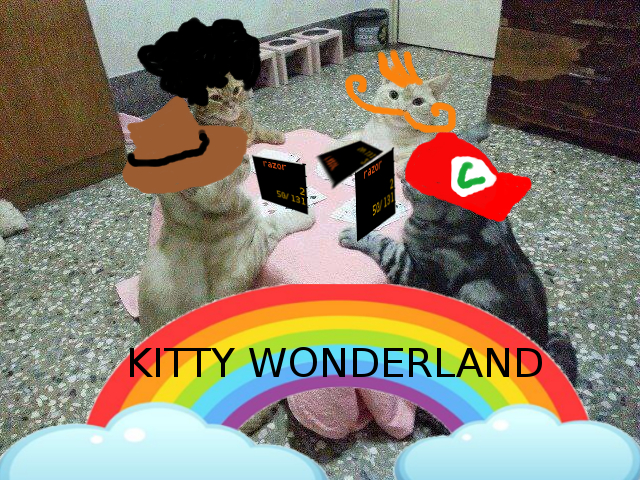
\includegraphics[width=\textwidth]{chats3.jpg}
\newpage
\tableofcontents

\newpage

\section{Nature du projet}
\subsection{Objectif}
Il s’agit dans ce projet de développer quelques mécanismes de base destinés à servir dans le développement d’un jeu.
Ce projet se découpera en différentes parties. Il nous est demandé dans un premier temps de mettre en place une version de base qui met en place un jeu de carte simple entre plusieurs joueurs. 
Les cartes pouvant infliger à l'adversaire des dégâts ou bien avantager le joueur la détenant.

Cette version sera améliorée au fur et a mesure des achievements.

\subsection{Cadre de travail}
Le projet est a effectuer en binôme, sous la tutelle d'un enseignant référent. Afin de gérer le travail en groupe, nous devons utiliser subversion, un outil de gestion des versions. Des heures de travail sont prévue sur l'emploi du temps le mardi et le vendredi après-midi pour nous permettre de réaliser ce projet. Notre enseignant référent sera là pour nous aider en cas de problème et pour valider les différentes étapes du projet.

\newpage
\section{Architecture du projet}
\subsection{Makefile}
Pour la compilation du projet et des tests, nous avons fait un Makefile par version. Nous avons ensuite fait un Makefile à la racine du projet qui appelle tous les Makefiles des sous-dossier avec une seule commande. 

Les commandes de notre Makefile sont: 
\begin{itemize}
\item make main: en règle par défaut qui compile toutes les versions de jeux
\item make test: qui compile et exécute tous les tests
\item make valgrind: qui permet de voir le retour de valgrind sur tout les tests
\item make clean: qui nettoie tout les exécutables et fichiers objets. 
\end{itemize}

\subsection{Structure}
Le projet se base sur plusieurs entités qui sont dépendantes entre elles. Le schéma suivant la structure globale de notre projet: 

\begin{figure}[!h]
\centering
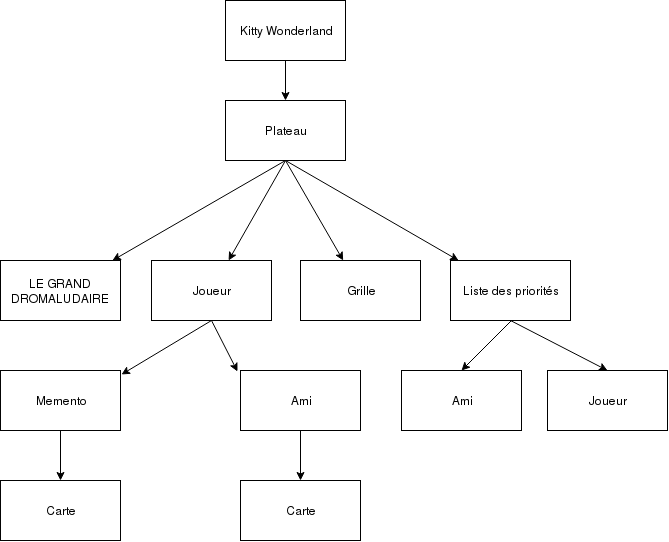
\includegraphics[width=\textwidth]{V6plus.png}
\caption{\label{fig:v_base}Diagramme de dépendance}
\end{figure}

On remarque que le plateau est a l'origine de la création de tout le jeux. En effet, c'est ce dernier gère la création de la grille de jeu, des joueurs, de la liste de priorités et du dromaludaire.
La liste des priorité va, quant a elle, gérer pour le plateau les listes d'amis et joueurs.
Nous avons aussi codé les amis afin qu'ils dépendent du joueurs qui les créent. En effet on peut les voir comme une invocation du joueur, la mort du joueur impactera sur ses amis en les tuant.
Les joueurs créent un mémento qui leur est propre et ce dernier est composé de cartes. L'ami, quant a lui, n'a qu'une seule carte.


\newpage
\section{Analyse technique}
\subsection{La version de Base}
La version de base du projet est une version simple du jeu de carte. On définit les principales structures du jeu, qui nous serviront tout au long du projet, à savoir les cartes, les joueurs et le plateau de jeu. 

\subsubsection{Stockage de la carte}
Le format de stockage de la carte est décrit ci dessous, il utilise une structure ayant comme champs un nom, un coût et une rareté.


\begin{verbatim}
struct carte{
   char* nom; 	
   int cout;
   int rarete;
};
\end{verbatim}

\subsubsection{Stockage du joueur}
Le joueur est lui aussi décrit a l'aide d'une structure de plusieurs champs.

\begin{verbatim}
struct joueur {
    int numero_joueur;
    int energie;
    int idee;
    int gain;
    int n_carte;
    carte *main;
};
\end{verbatim}

Le numéro du joueur va permettre son identification par la suite. Le joueur aura la possibilité de jouer une carte en fonction de ses champs énergie, idée et gain. Les cartes de sa main seront représentées par un tableau de carte ainsi qu'un nombre de cartes. 

\subsubsection{Stockage du plateau de jeu}
Enfin le plateau de jeu est représente par une structure comprenant un nombre de joueurs au départ du jeu, le nombre de joueurs vivants a un instant défini pendant la partie, ainsi qu'un tableau de joueurs et de classement permettant d'afficher les résultats a la fin de la partie.

\begin{verbatim}
struct plateau_de_jeu {
    int nb_joueur;
    int nb_joueur_vivant;
    joueur* tab_joueur;
    int* classement_joueur;
};
\end{verbatim}


Pour la version de base, le jeu fonctionne ainsi :
Les joueurs jouent chacun leurs tours, ils jouent une carte aléatoirement dans leur main et le plateau de jeu la traitera. Cette carte sera par la suite supprimé et lorsque le joueur piochera, une nouvelle carte sera créée aléatoirement. Le dernier joueur en vie gagne.

\newpage
\subsection{Version 1 : Ajout de mémento}
La version 1 change la façon dont les cartes sont piochées. Au lieu de créer de façon aléatoire les cartes, les joueurs vont désormais piocher leurs cartes dans un paquet de carte, ou mémento. 

Ce mémento se composera de 50 cartes créées aléatoirement au début de la partie en fonction de leur probabilité.
Ce mémento sera géré comme une FIFO (First In First Out). En effet lorsque le joueur déposera une carte, ce dernier le fera à la fin du mémento et par la suite il piochera la première carte du mémento.

Nous avons choisi d'implémenter le mémento à l'aide d'une liste doublement chaînée. 
Nous avons créé 2 structures pour y parvenir. 

La première représentant la tête de liste:
\begin{verbatim}
struct memento_list {
    int longueur;
    memento premier;
    memento dernier;
};
\end{verbatim}

Et la seconde représente les entités de cette liste:
\begin{verbatim}
struct memento {
    memento precedent;
    memento suivant;
    carte c;
};
\end{verbatim}

Un mémento contient une carte avec un pointeur sur le mémento suivant et un pointeur sur le mémento précédent.
Une mémento\_list contient deux pointeur, un sur la tête de liste et l'autre sur la queue de liste. 

Nous avons également modifié la structure joueur afin de lui ajouter une memento\_list. 

Ce choix de modélisation s'adapte parfaitement au projet. Il nous permet d'effectuer facilement les tâches telles que ajouter une carte et retirer une carte. 

\begin{figure}[!h]
\centering
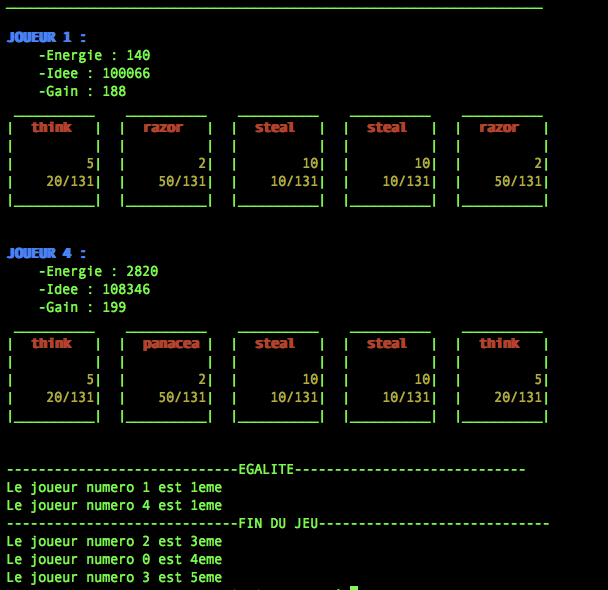
\includegraphics[width=8cm]{version1.png}
\caption{\label{fig:v_base}Extrait du jeu de version1}
\end{figure}

\newpage
\subsection{Version 2 : La grille de jeu}
La version 2 ajoute une grille de jeu sur laquelle les joueurs vont se déplacer à chaque tour. 

Deux nouvelles structures ont été implémenté. 
La structure position stocke les coordonnées x et y d'un joueur.
\begin{verbatim}
struct position {
    int x;
    int y;
};
\end{verbatim}

La seconde rassemble tout les champs permettant d'utiliser une grille de jeu.
\begin{verbatim}
struct grille_de_jeu {
    bool** tab;
    int nb_joueur;
    struct position* tab_position_actuelle;
    struct position* tab_position_futur;
};
\end{verbatim}

La structure position permet de placer un joueur sur la grille. 
Il est défini par 2 entiers correspondant aux coordonnées x et y dans un tableau a 2 dimensions. Cette structure position devient donc un champs de la structure du joueur. 

La grille de jeu est définie par un tableau à 2 dimensions de booléens. Ces booléens correspondent à l'état des cases, vrai pour une case libre, faux pour une case occupée. 

Le nombre de joueur sert à savoir combien de joueurs jouent. 
Ce champ nous donne le nombre de cases de nos tableaux de positions actuelles et de positions futurs. 
Le tableau tab\_position\_actuelle contient les positions des joueurs au début du tour de jeu. 
Le tableau tab\_position\_futur stocke les positions des joueurs après déplacement.
Ces deux tableaux sont essentiels afin de gérer les collisions, en effet lorsque les positions futures sont identiques les joueurs reviennent a leur position de début de tour.

La grille est une grille torique, ce qui signifie que l'on peut se représenter la grille comme une sphère, il n'y a aucune limite de bordures de grille \ref{grille}.

À chaque tour, les joueurs se déplacent d'un nombre de case compris entre 0 et 5 dans toutes les directions. 
La façon la plus simple de traiter cette zone de déplacement est de créer une fonction qu'y gère le déplacement d'une seule case et d'appeler cette fonction un nombre aléatoire de fois. 

\begin{figure}[h]
	\centering
    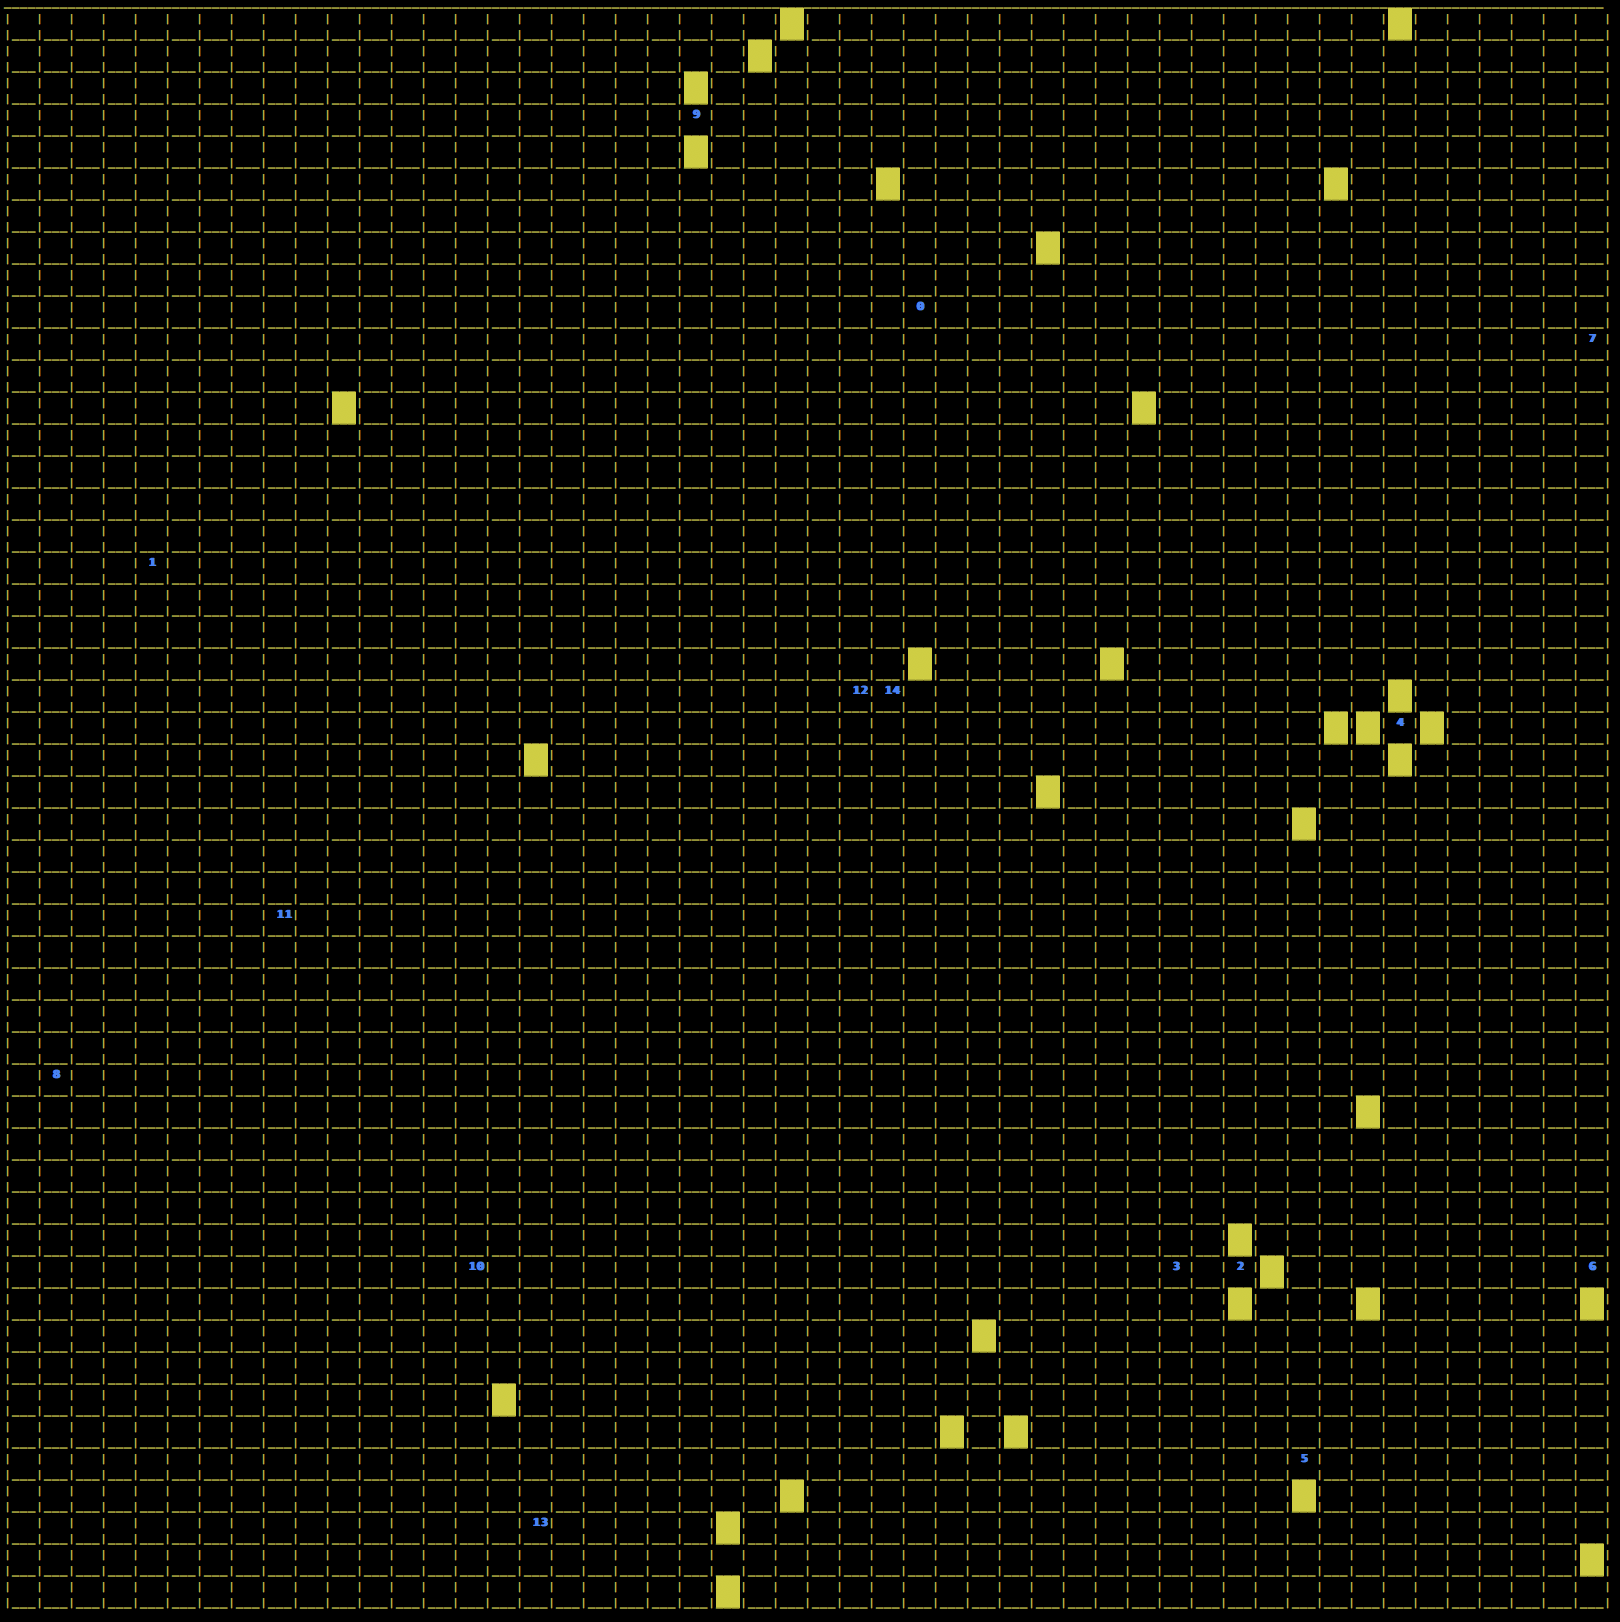
\includegraphics[width=9cm]{grille.png}
    \caption{\label{grille} Extrait d'affichage de la grille}
\end{figure}


\newpage
\subsection{Version 3 : Les amis des Kitty Cats}
Dans le troisième achievement, il faut implémenter une nouvelle carte, qui fait apparaître un ami sur le terrain. Un ami est une sorte de joueur qui possède une seule carte et qui vise un adversaire en particulier. 
L'ami est représenté par la structure suivante : 
\begin{verbatim}
struct ami {
    int numero_adversaire;
    int numero_ami;
    int numero_joueur;
    int vie;
    int energie;
    int idee;
    int gain;
    carte c;
    struct position position;
};
\end{verbatim}

Le numero\_adversaire correspond à l'adversaire visé, le numero\_joueur correspond au joueur qui l'a fait apparaître, et numero\_ami est l'identifiant de l'ami. 

Un ami peut être considéré comme un joueur particulier excepté qu'il a une durée de vie.  En effet son champ vie est initialisé a 20 et correspond au nombre de tour restant avant de mourir.

Nous avons considéré l'ami comme une invocation faite par le joueur. Un joueur peut donc se créer des amis et ces amis peuvent eux aussi en créer, ils seront alors rattachés au même joueur.  

L'ami a un numéro de joueur cible qu'y lui est attribué a sa création. Or, il a fallu gérer le cas ou ce joueur est mort. Lorsque cette configuration de jeux arrive, le joueur en charge de l'ami lui réinitialise sa cible avec son adversaire actuel.

Nous avons mis a jour notre affichage pour inclure les amis dans l'affichage des cartes\ref{carteAmi} et sur la grille.\ref{grilleAmi}

\begin{figure}[h]
    \begin{minipage}[c]{0.4\linewidth}
        \centering
        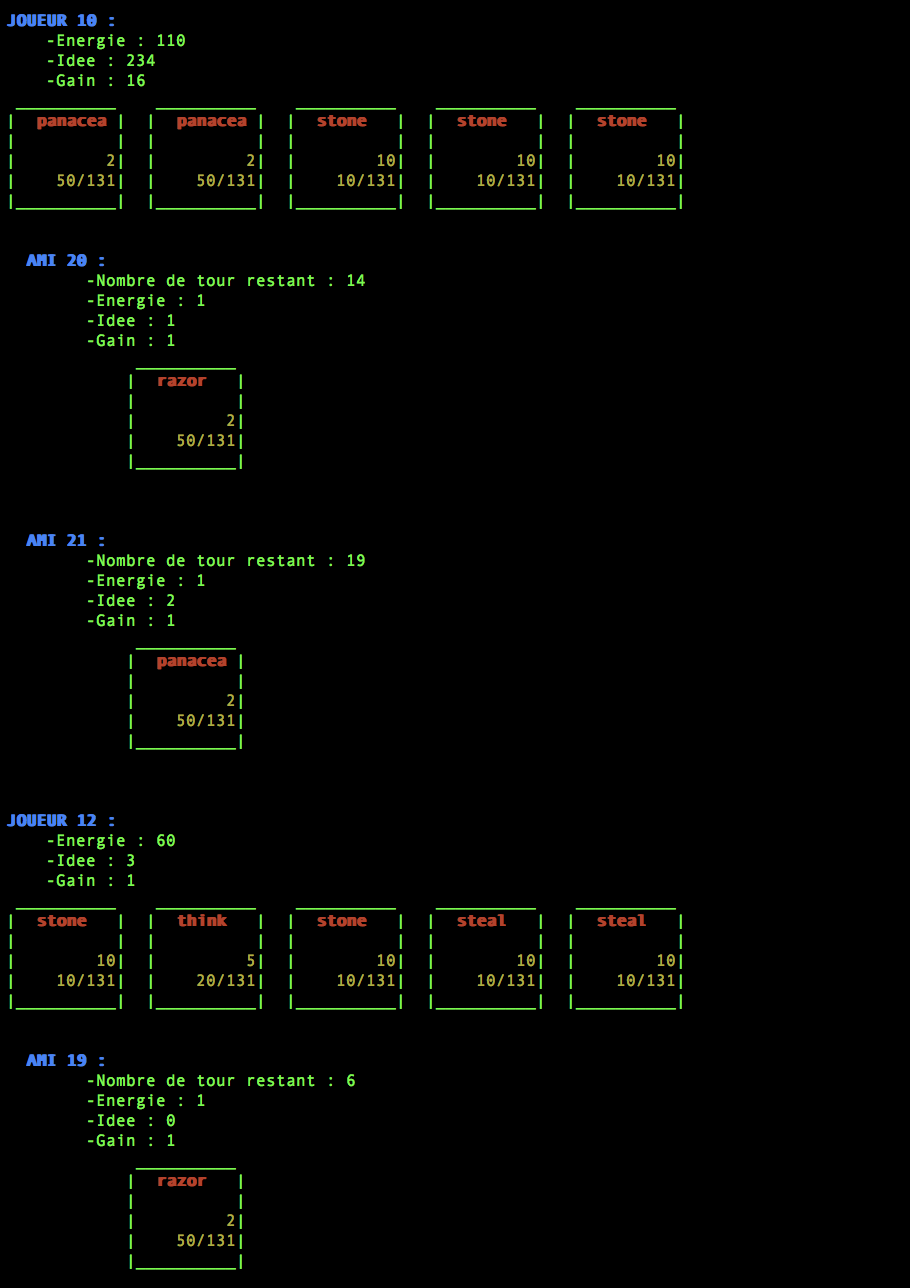
\includegraphics[width=7cm]{ami.png}
        \caption{\label{carteAmi} Affichage des cartes des joueurs et amis}
    \end{minipage}
    \hfill%
    \begin{minipage}[c]{0.48\linewidth}
        \centering
        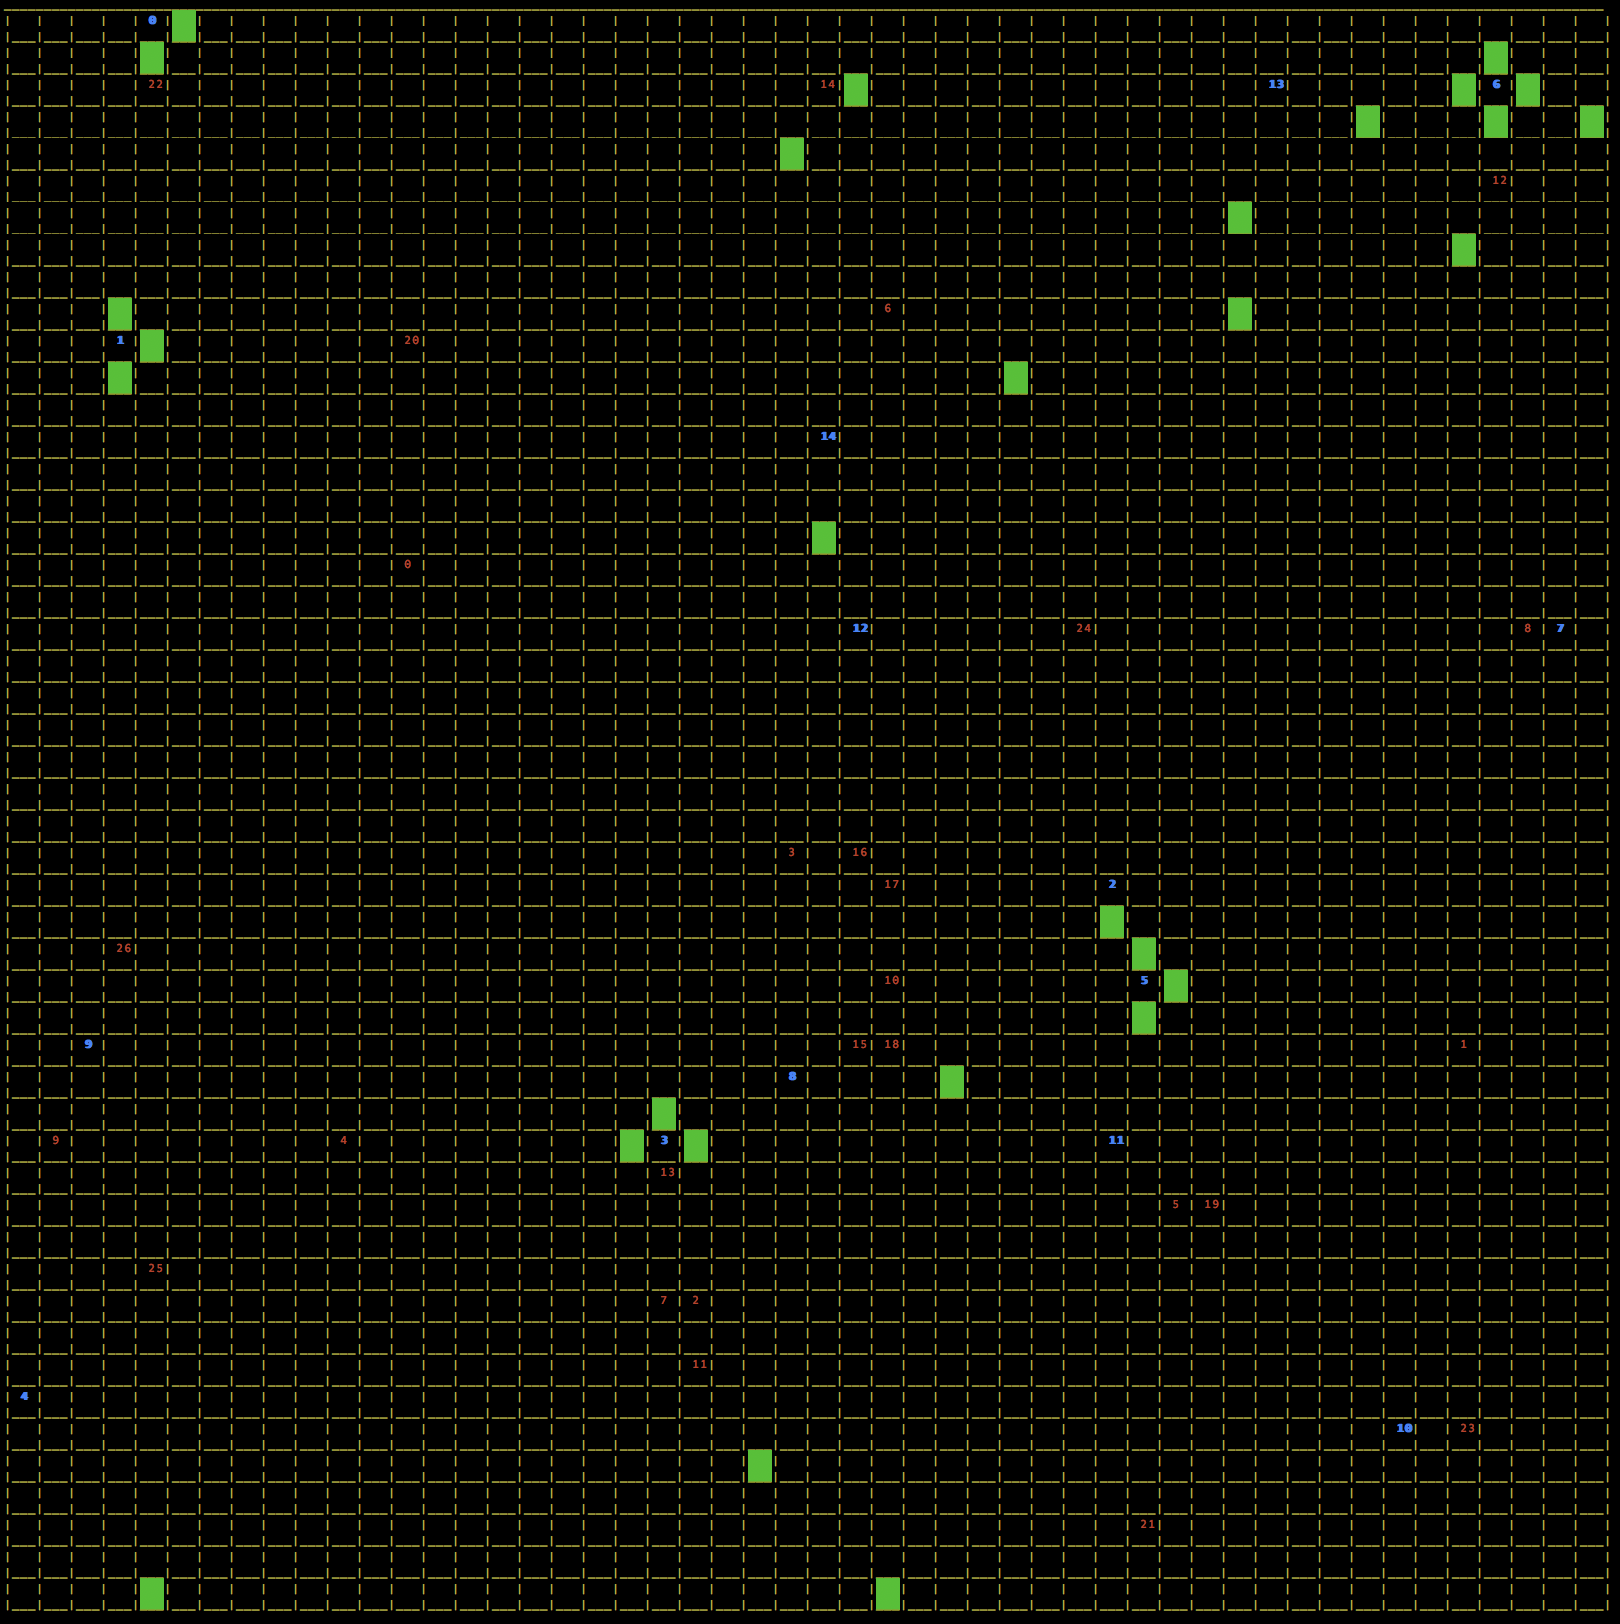
\includegraphics[width=10cm]{grille_a.png}
        \caption{\label{grilleAmi} Affichage de la grille avec amis en rouge}
    \end{minipage}
\end{figure}

\newpage
\subsection{Version 4 : Généricité}
Pour la version 4, il nous est demandé de traiter les cartes par des pointeurs de fonction au lieu d'utiliser des switch/case ou des if/else if. 
Nous avons donc défini un type pointeur\_fonction 
\begin{verbatim}
typedef void (*pointeur_fonction)(int j, int ad, bool ami, int num_ami);
\end{verbatim}
et ajouté un pointeur de fonction dans la structure de carte. 
\begin{verbatim}
struct carte {
    char* nom;
    int cout;
    int rarete;
    pointeur_fonction application_carte;
};
\end{verbatim}

Nous avons ensuite créé une fonction propre à chaque carte, toutes avec la même signature, par exemple :

\begin{verbatim}
void kitty_think(int moi, int ad, bool ami, int num_a) {
    // on gère si la carte est jouée par un joueur ou un ami 
    if (ami == false) {
        set_gain(get_joueur(moi), get_gain(get_joueur(moi)) + 1);
        set_idee(get_joueur(moi), get_idee(get_joueur(moi)) - 5);
    } else {
        augmenter_gain(get_ami(num_a, get_joueur(moi)));
        diminuer_idee(get_ami(num_a, get_joueur(moi)), 5);
    }
}
\end{verbatim}

La fonction traiter\_carte est ainsi allégée et ne contient plus que l'utilisation du pointeur de fonction. 

\subsection{Version 5: Vitesse des chatons}
La version 5 ajoute une nouvelle notion, la notion de temps. Chaque action coûte un temps, et les joueurs qui jouent à chaque tour sont ceux ayant le moins de temps. 


Pour implémenter ça, nous avons créé liste de priorité \ref{priorite}. Cette liste est en fait une liste de liste.
Elle contient donc une tête de liste pointant sur la premier priorité e la liste et sur la dernière. Chaque entité de cette liste appelé priorité, est en fait une tête de liste vers une nouvelle liste doublement chaînée contenant les joueurs ou amis. 


Tous les joueurs avec le moins de temps sont dans la première priorité, tous les joueurs avec le deuxième plus petit temps dans la deuxième etc...
Tous les joueurs d'une même priorité jouent donc en même temps.

Une fois le tour du joueur terminé, nous calculons son nouveau temps et nous l'insérons dans la priorité correspondante.  

\begin{figure}[!h]
\centering
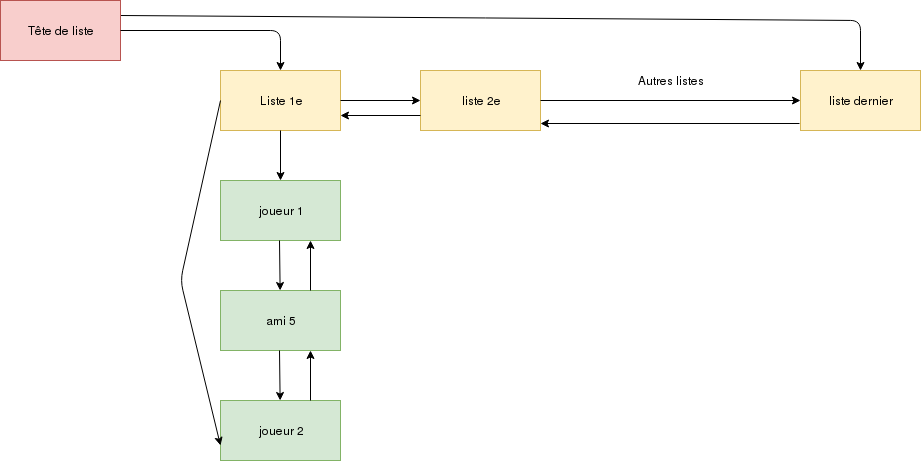
\includegraphics[width=.8\textwidth]{priorite.png}
\caption{\label{priorite}Schéma de la liste de priorité}
\end{figure}
Pour utiliser une liste, nous commençons par extraire la première liste.\ref{coup1}. 
\begin{figure}[!h]
\centering
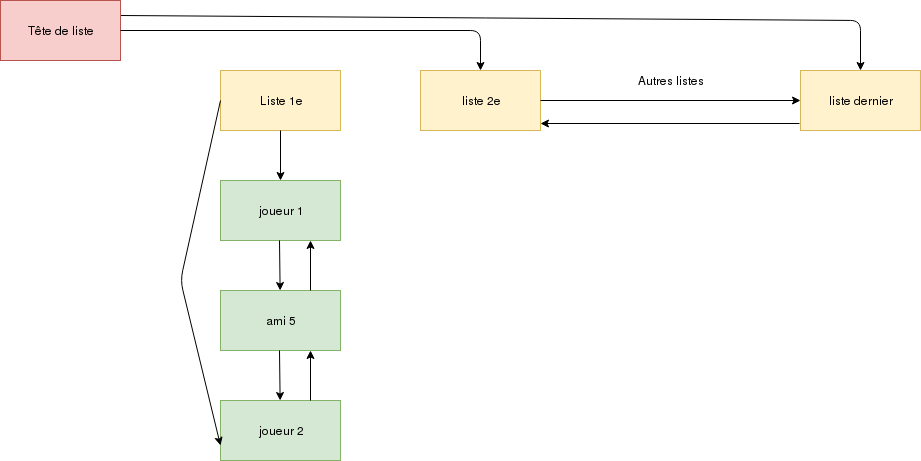
\includegraphics[width=.8\textwidth]{coup1.png}
\caption{\label{coup1}Extraction de la première liste}
\end{figure}
Ensuite nous extrayons les joueurs un par un afin de les faire jouer. 
\ref{coupe2}
\begin{figure}[!h]
\centering
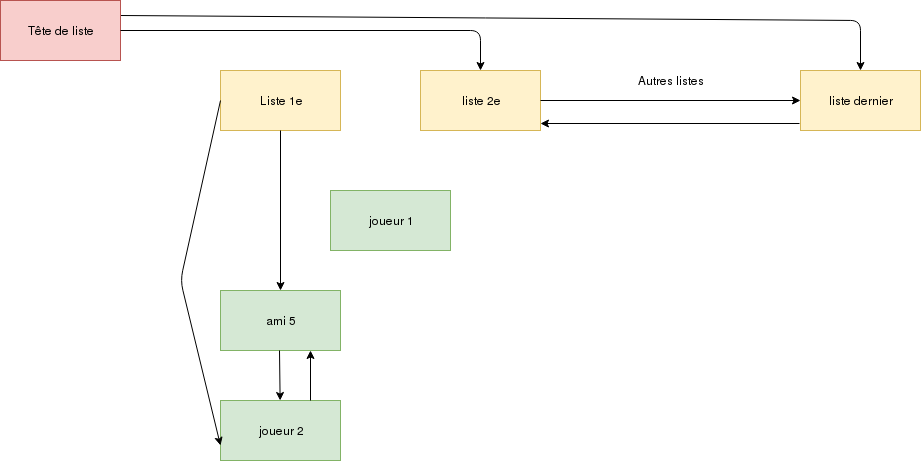
\includegraphics[width=.8\textwidth]{coupe2.png}
\caption{\label{coupe2}Extraction du premier joueur afin le faire jouer}
\end{figure}


Nous avons fait les choses ainsi plutôt qu'une liste chaînée simplement car on parcours moins de priorité pour trouver la place du joueur et l'insertion de ce dernier est moins coûteuse. 

\newpage
\subsection{Version 6 : LE GRAND DROMALUDAIRE}
Cette version du projet n'a pas été terminer faute de temps. Néanmoins nous avons réfléchi à la façon ont nous aurions pu résoudre le problème posé.
Le problème de déplacement du dromaludaire n’était pas un obstacle puisque nous avions toutes les fonctions utiles déjà implémentées dans nos autres versions.
En effet, nous aurions fait le déplacement de ce dernier d'une case en une case en vérifiant qu'il n'y ai pas collisions avec un joueur ou un ami et en ne traitant pas le fait qu'il y ai un caramel mous. 

Au début de leur tour de jeu, les joueurs ou amis auraient vérifié le fait qu'il ne soit pas collé au dromaludaire. Si jamais ça avait été le cas, il aurait défausser sa main grâce a une fonction déjà implémentée puis pour résoudre le problème des 5 kitty cartes "think" nous aurions mis en place un compteur qui serait initialisé à 0 à la création du joueur, puis serait passer à 5 au contact du dromalutaire.

A partir de ce moment la, le joueur ayant ce compteur différent de 0, décrémentera ce dernier à chaque tour, tout en feignant le traitement d'une carte kitty think. Des lors que le compteur est à 1 en début de tour le joueur traitera sa dernière carte kitty think puis piochera 5 nouvelles cartes de son mémento. 



\newpage
\section{Tests}
Les tests constituent une partie importante du projet. Ils permettent de s'assurer que le code fonctionne, et permettent également de ne pas faire de régression en passant d'une version à l'autre. 

Pour fabriquer notre programme de test, nous avons créé des fonctions de test pour chaque fonction de notre projet (hors affichage, getters et setters). Chacune de ces fonctions appelle la fonction qu'elle teste dans un contexte maîtrisé et vérifie que la fonction effectue bien ce qu'elle est censé faire. Par exemple la fonction test\_creer\_carte() créé une carte de chaque type, et vérifie que cette carte possède bien les bons attributs. La fonction retourne un booléen, TRUE si le test est bon, FALSE sinon. 

Le main du programme de test appelle toutes les fonctions de test et fait un "AND" bit à bit des retours de ces fonctions, ainsi si la moindre fonction de test ne marche pas, le test ne passera pas. 

Une fonction de test qui retourne FALSE enverra un message sur le terminal indiquant qu'il y a un problème afin de pouvoir détecter les fonctions qui ne marchent pas. Un test qui passe nous gratifiera d'un magnifique "YOUPI tout passe!" en vert. 

\begin{figure}[!h]
\centering
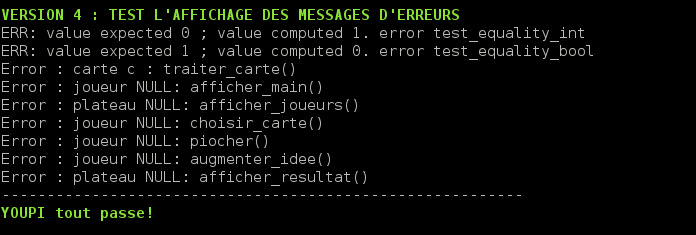
\includegraphics[width=\textwidth]{CaptureTest.png}
\caption{\label{fig:v_base}Exemple d'un test qui passe}
\end{figure}

\newpage
\section{Analyse Valgrind}
Pour effectuer ce projet, nous avons utilisé l'allocation dynamique grâce à la fonction malloc. De ce fait, il est important que nos allocations soient libérées une fois le programme terminé. Pour nous assurer qu'aucune fuite mémoire ne puisse arriver, nous avons utilisé Valgrind. Valgrind est un outil qui permet de mettre en évidence les fuites mémoires.
\subsection{Sur notre exécutable de la version de base}
\begin{figure}[!h]
\centering
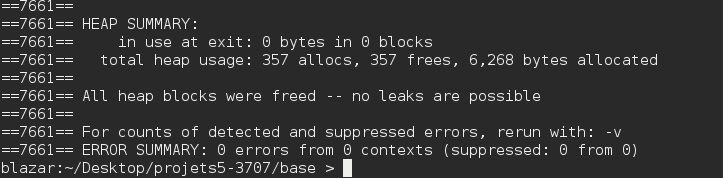
\includegraphics[width=\textwidth]{valgrind_base.png}
\caption{\label{fig:v_base}Valgrind sur notre exécutable base}
\end{figure}

\subsection{Sur notre exécutable de la version 1}
\begin{figure}[!h]
\centering
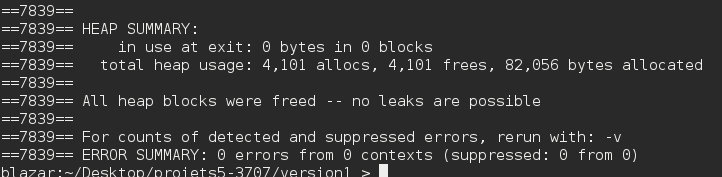
\includegraphics[width=\textwidth]{valgrind_version1.png}
\caption{\label{fig:v_base}Valgrind sur notre exécutable de la première version}
\end{figure}

\subsection{Sur notre exécutable de la version 2}
\begin{figure}[!h]
\centering
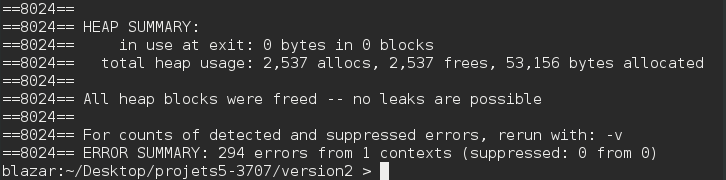
\includegraphics[width=\textwidth]{valgrind_version2.png}
\caption{\label{fig:v_base}Valgrind sur notre exécutable de la deuxième version}
\end{figure}

\subsection{Sur notre exécutable de la version 3}
\begin{figure}[!h]
\centering
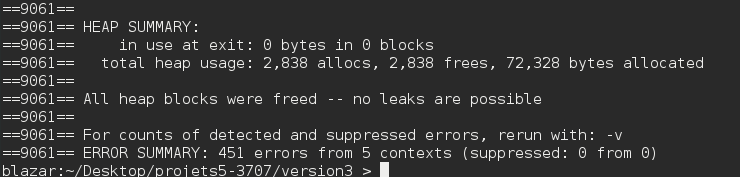
\includegraphics[width=\textwidth]{valgrind_version3.png}
\caption{\label{fig:v_base}Valgrind sur notre exécutable de la troisième version}
\end{figure}

\newpage
\section{Bilan}
Au terme de ces 6 semaines, nous pouvons dire que le premier projet de programmation a été pour nous une expérience enrichissante sur plusieurs plans. 

Tout d'abord sur le plan technique, ce projet nous a permis de développer nos compétences et de mettre en application les cours d'environnement de travail et de programmation impérative en C. Nous avons également appris à nous servir de subversion pour bien gérer les différentes versions de notre projet.  

La gestion du groupe est un autre aspect important de ce projet. En effet, travailler en groupe nécessite une répartition des tâches efficace. Ceci demande une bonne organisation ainsi qu'une bonne communication afin que le groupe puisse fonctionner dans les meilleures conditions. 


\end{document}
